\section{Real Data}

\subsection{Data Structure}

The data given by the industrial partner has been anonymised due to confidentiality agreements, and thus neither the type of the variables nor nature of the data can be disclosed. The information which can be disclosed, however, is that the raw data consisted of 979 observations of 9 variables, with the ninth variable being the one of interest. The form of the raw data was such that it was a series of panels stacked in a single column, and the frequency of the observations was quarterly (i.e. four times a year). Due to the way the statistical packages were programmed, a minimum of 8 observations had to be imposed on the data, so series which had less than 8 observations were removed. The cleaned data was therefore 36 time series: one with a length of 40, four of length 39, and then one each from lengths 38 to 8.

\subsection{Data Characteristics}

As stated, the structure of the cleaned data was a number of panels consisting of of time series, with observations ranging from 40 to 8. Before summary statistics were calculated, all the series were correctly graphed by the corresponding quarter, as seen in Graph 1.

To determine which model the data followed (zero-mean, mean or trend), a dummy variable range from one to the length of the series was regressed upon each series and the p-values for both the trend and intercept were analyzed. Of the 36 series remaining after the cleaning phase, 29 were found to have a trend at a 95\% confidence and 30 at a 90\% confidence. As stated previously, the data is assumed to have the same Data-Generating Process, ergo the remaining series which did not have high enough confidence values for the intercept term are assumed to have a trend in the DGP.

%\begin{figure}
	
%\includegraphics[scale=0.5]{paneldata.jpg}

%\end{figure}


\begin{figure}[htp]
	\centering
	\begin{subfigure}{0.75\textwidth}
		\centering
		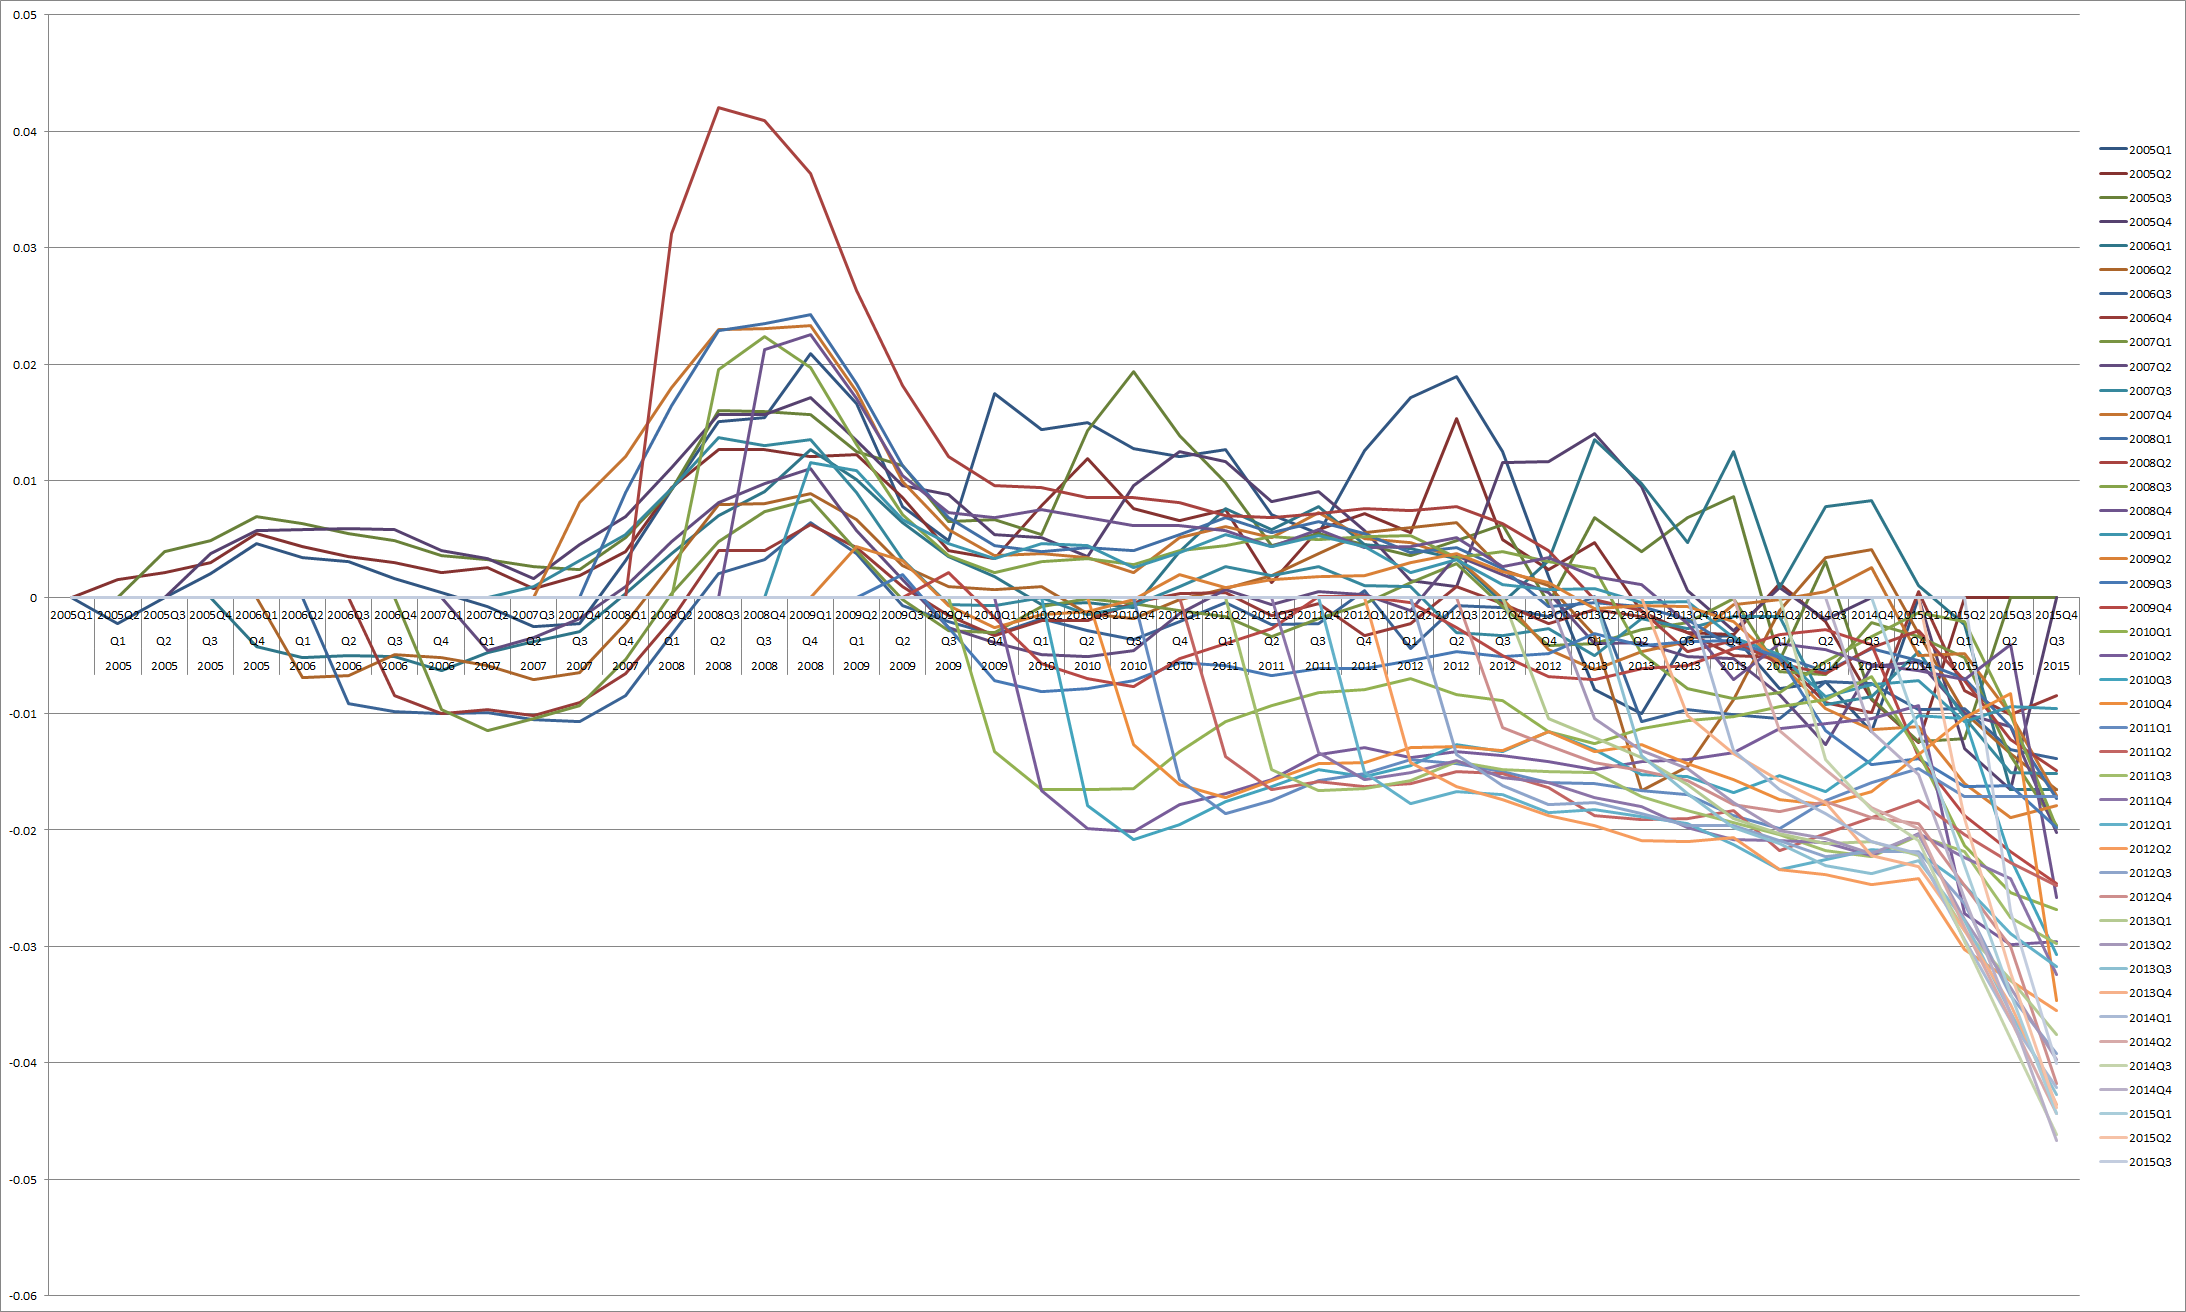
\includegraphics[width= \linewidth]{panel_graph}
	\end{subfigure}
\caption{Time series plot of all real data.}
\end{figure}

After the model was identified as having a linear trend, the next step was to identify whether or not it followed an $AR$ process. All the series were passed through the auto-correlation function and partial-auto-correlation function. On balance, the individuals all followed an autoregressive process of order one, as is visible with some of the selected ACF/PACF graphs shown below. 


\begin{figure}[htp]
	\centering
	\begin{subfigure}{0.23\textwidth}
		\centering
		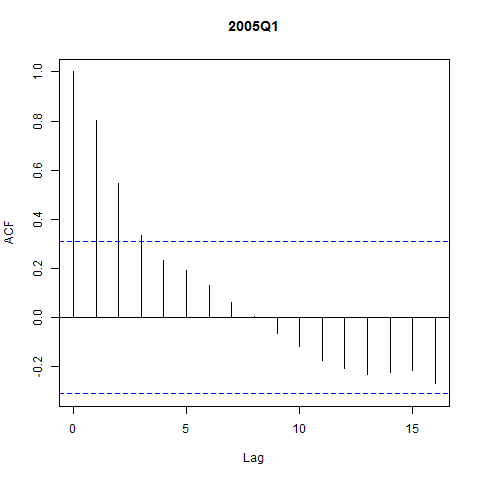
\includegraphics[width= \linewidth]{2005Q1-acf}
	\end{subfigure}
	\begin{subfigure}{0.23\textwidth}
		\centering
		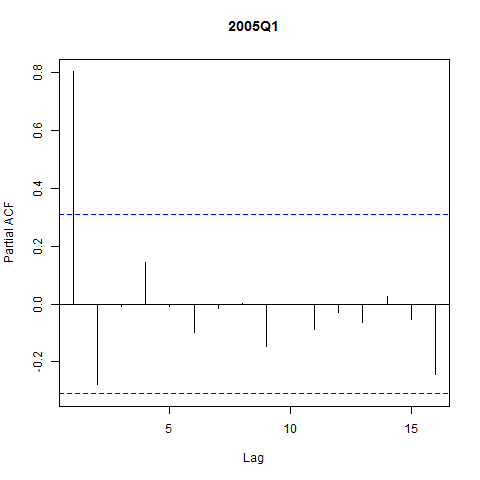
\includegraphics[width=\linewidth]{2005Q1-pacf}
	\end{subfigure}
	\begin{subfigure}{0.23\textwidth}
		\centering
		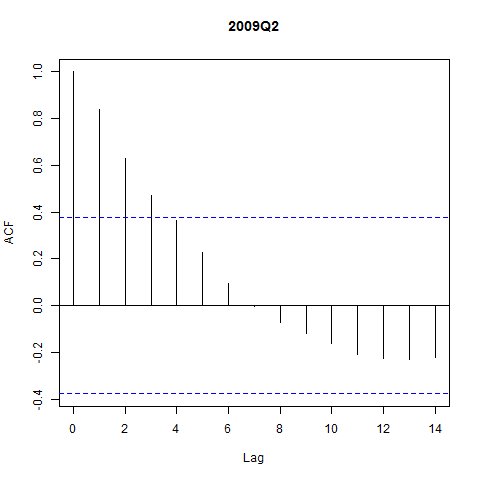
\includegraphics[width= \linewidth]{2009Q2-acf}
	\end{subfigure}
	\begin{subfigure}{0.23\textwidth}
		\centering
		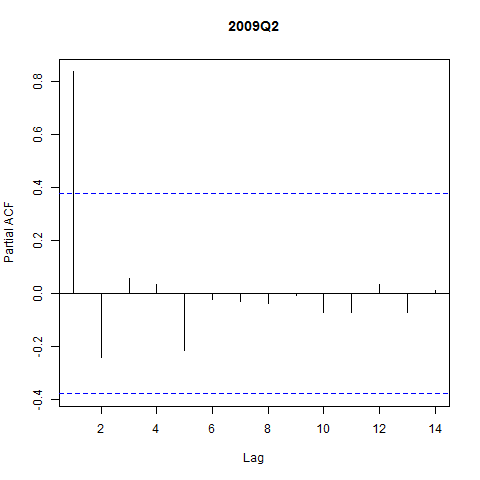
\includegraphics[width=\linewidth]{2009Q2-pacf}
	\end{subfigure}
\caption{Select ACF and PACF plots from the real data.}
\end{figure}

Again, it should be noted that the data did not uniformly show an $AR(1)$ process on the ACF/PACF graphs, but because the individuals of the panel are assumed to be samples of an identical process, it is further assumed that the few series which are not appearing as $AR(1)$ process are appearing as such due to sampling error, which is further justified by the fact that these non-conforming series are the shortest lengths, i.e. smallest sample size.


\section{Simulated Data}

\subsection{Data Structure}

The panels created for the Monte Carlo simulations ranged from a panel with 8 observations of 2 individuals to 25 observations of 50 individuals. Each individual was a bespoke AR(1) process with a $\rho$ value as specified in that instance.


\subsection{Data Characteristics}

The data used in the Monte Carlo simulations was an AR(1) process, which was simulated using R. The process can be expressed as below:

\begin{equation}
y_t = \rho y_{t-1} + \epsilon_t
\end{equation}

A range of $\rho$ values was simulated, from 0.5 to 1, in order to gauge the power of the tests. All but the last value ($\rho = 1$) are stationary time series, with the exception being non-stationary with a unit-root. With low values of $\rho$, the series is clearly deterministic around a mean (which in this case is zero) with a small degree of noise. Four sample processes are displayed below where the value of $\rho$ has been set for 0.5 and T is 10,20,100,500.

\begin{figure}[htp]
	\centering
	\begin{subfigure}{0.23\textwidth}
		\centering
		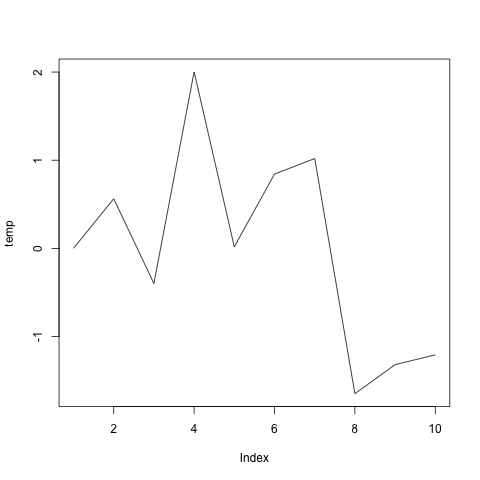
\includegraphics[width= \linewidth]{10-05-plot}
	\end{subfigure}
	\begin{subfigure}{0.23\textwidth}
		\centering
		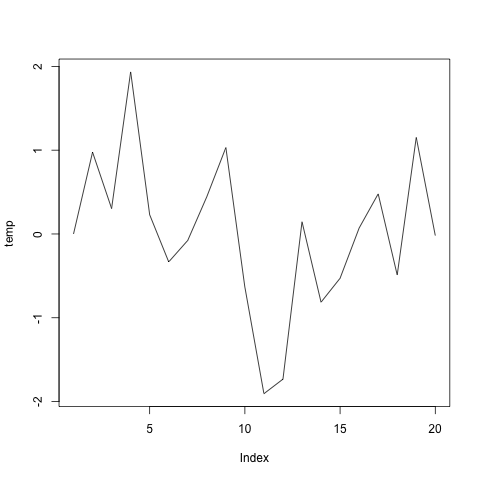
\includegraphics[width=\linewidth]{20-05-plot}
	\end{subfigure}
	\begin{subfigure}{0.23\textwidth}
		\centering
		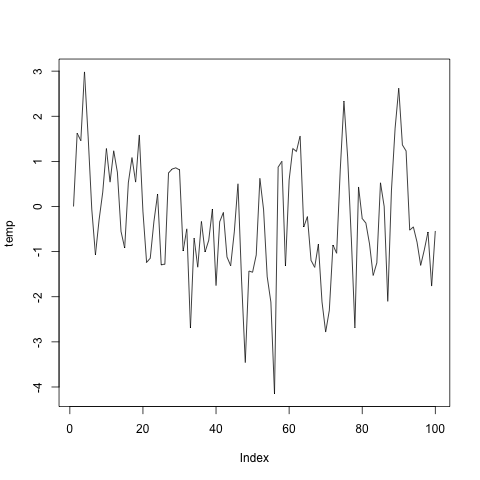
\includegraphics[width= \linewidth]{100-05-plot}
	\end{subfigure}
	\begin{subfigure}{0.23\textwidth}
		\centering
		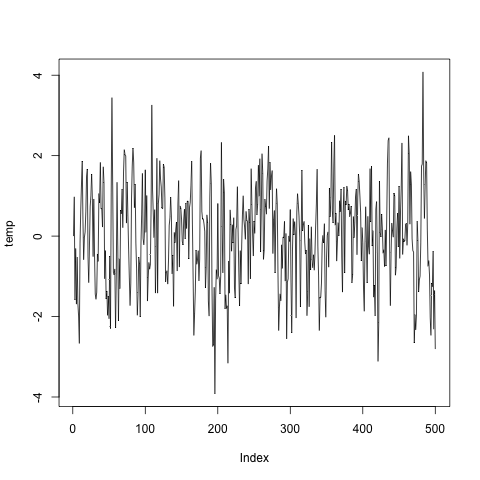
\includegraphics[width=\linewidth]{500-05-plot}
	\end{subfigure}
\caption{Time series plots for $\rho = 0.5$}
\end{figure}



Even for the processes with $T = 10$ and $T = 20$, the zero-mean trend is clearly visible, albeit with a large degree of noise. When $T = 100$ or $500$, however, the process very clearly appears stationary around a zero mean. When the ACF and PACF are applied to the data, they detect no auto-correlation for cases with $T = 10$ and $T = 20$, while for the case of $T = 100$, it is borderline and for $T = 500$ it is clear cut, as is shown in the charts below.

\begin{figure}[htp]
	\centering
	\begin{subfigure}{0.23\textwidth}
		\centering
		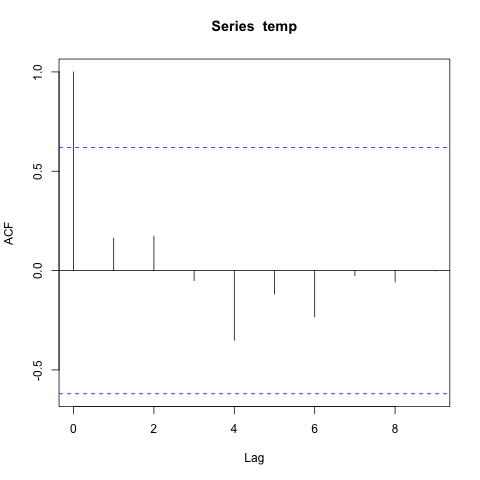
\includegraphics[width= \linewidth]{10-05-acf}
	\end{subfigure}
	\begin{subfigure}{0.23\textwidth}
		\centering
		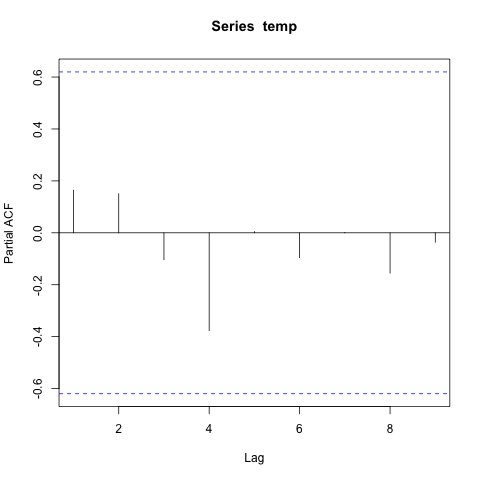
\includegraphics[width=\linewidth]{10-05-pacf}
	\end{subfigure}
	\begin{subfigure}{0.23\textwidth}
		\centering
		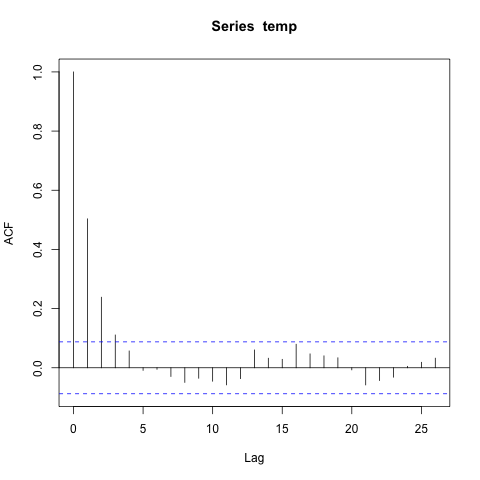
\includegraphics[width= \linewidth]{500-05-acf}
	\end{subfigure}
	\begin{subfigure}{0.23\textwidth}
		\centering
		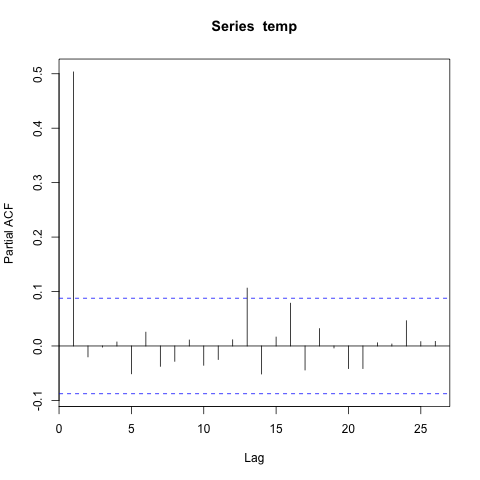
\includegraphics[width=\linewidth]{500-05-pacf}
	\end{subfigure}
	\caption{ACF and PACF plots for $\rho = 0.5$}
\end{figure}


This mirrors the issue motivating this thesis: with short time series, even thought the underlying process has a certain characteristic (in this case, that characteristic is serial correlation in the errors), these characteristics are undetectable with classic tests due to the short length. This first case can be compared to a series of processes with identical lengths, but where $\rho = 0.75$ instead of 0.5. 

\begin{figure}[htp]
	\centering
	\begin{subfigure}{0.23\textwidth}
		\centering
		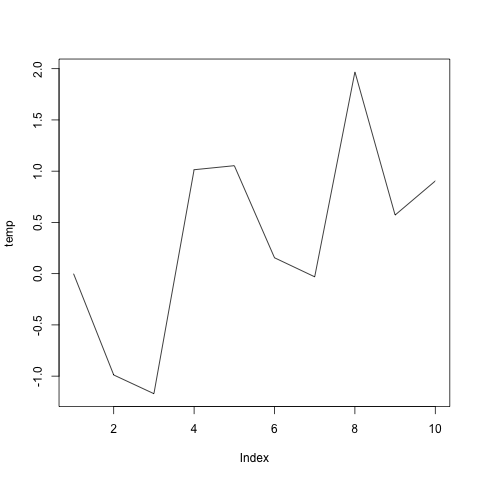
\includegraphics[width= \linewidth]{10-075-plot}
	\end{subfigure}
	\begin{subfigure}{0.23\textwidth}
		\centering
		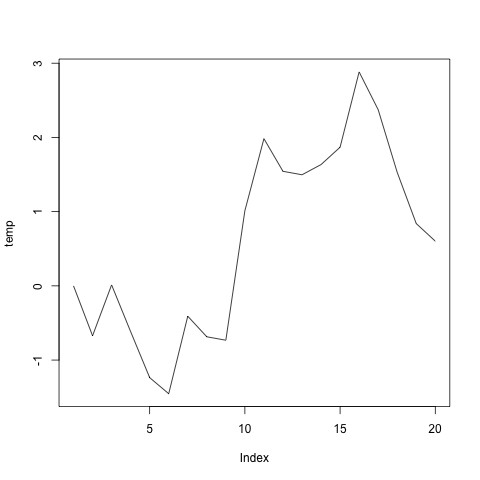
\includegraphics[width=\linewidth]{20-075-plot}
	\end{subfigure}
	\begin{subfigure}{0.23\textwidth}
		\centering
		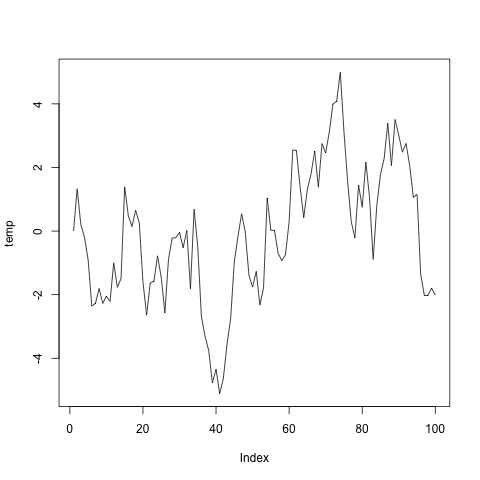
\includegraphics[width= \linewidth]{100-075-plot}
	\end{subfigure}
	\begin{subfigure}{0.23\textwidth}
		\centering
		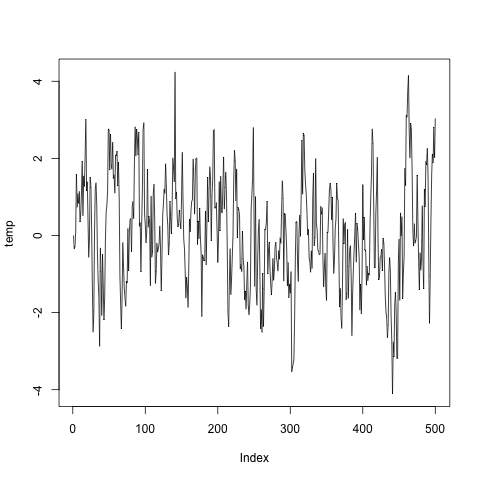
\includegraphics[width=\linewidth]{500-075-plot}
	\end{subfigure}
\caption{Time series plots for $\rho = 0.75$}
\end{figure}



The differences between the two processes are clear, the first process ($T=10$) appears largely stochastic while T = 20 is deterministic with very large residuals. Even $T = 100$ appears to be non-stationary, and it is only when $T = 500$ that the underlying process becomes clear and stationary around a zero mean. The ACF and PACF are likewise different in this case. The ACF for T = 10 does not indicate autocorrelation, but $T = 20$ does slightly so, and $T = 100$ and $T = 500$ exhibit very strong autocorrelation in the ACF. With the PACF behaves similarly, with $T = 10$ indicating no lags, while $T = 20$ indicates (wrongly) an AR(2) process. $T = 100$ and $T = 500$ correctly identify an AR(1) process with the PACF, as is shown below.

\begin{figure}[htp]
	\centering
	\begin{subfigure}{0.23\textwidth}
		\centering
		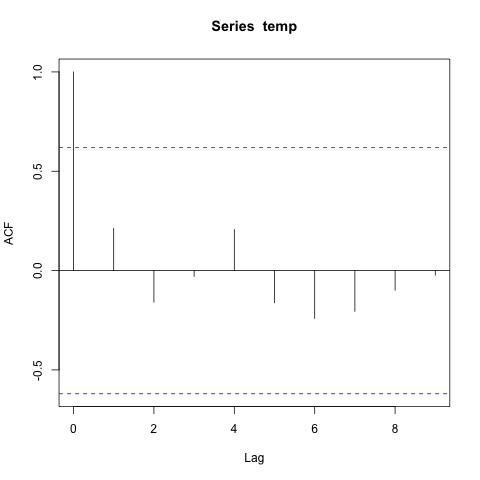
\includegraphics[width= \linewidth]{10-075-acf}
	\end{subfigure}
	\begin{subfigure}{0.23\textwidth}
		\centering
		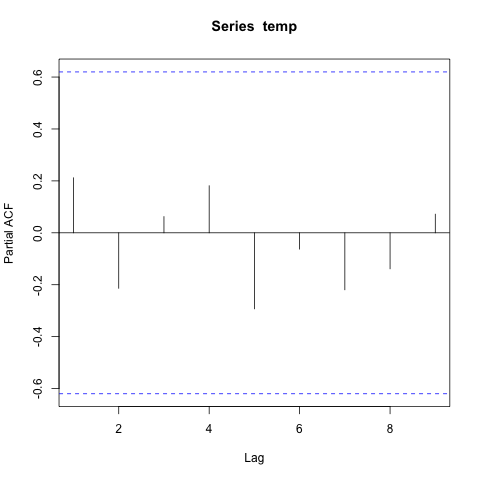
\includegraphics[width=\linewidth]{10-075-pacf}
	\end{subfigure}
	\begin{subfigure}{0.23\textwidth}
		\centering
		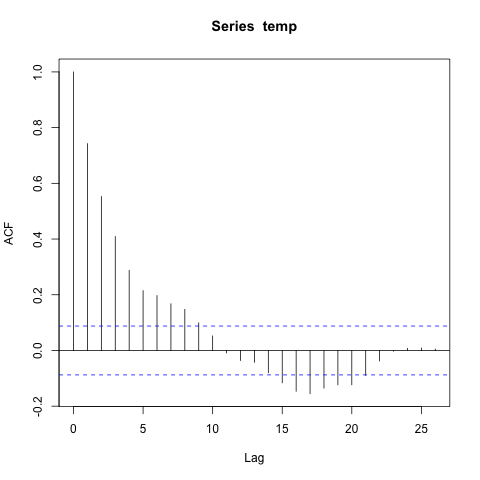
\includegraphics[width= \linewidth]{500-075-acf}
	\end{subfigure}
	\begin{subfigure}{0.23\textwidth}
		\centering
		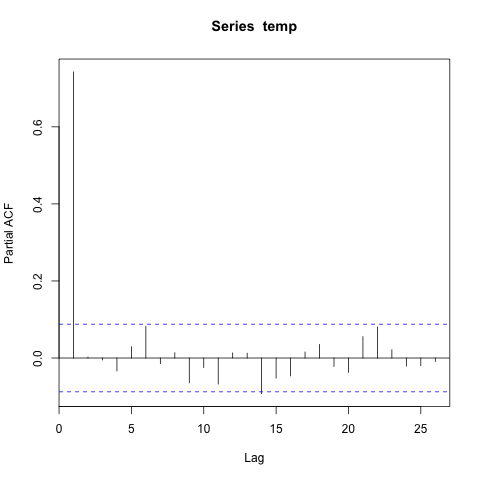
\includegraphics[width=\linewidth]{500-075-pacf}
	\end{subfigure}
\caption{ACF and PACF plots for $\rho = 0.75$}
\end{figure}


Moving further towards a unit root, a process with $\rho = 0.9$ behaves even more stochastically than the previous two processes.

\begin{figure}[htp]
	\centering
	\begin{subfigure}{0.23\textwidth}
		\centering
		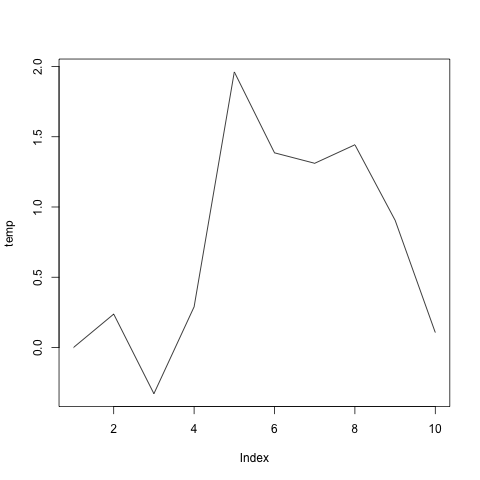
\includegraphics[width= \linewidth]{10-09-plot}
	\end{subfigure}
	\begin{subfigure}{0.23\textwidth}
		\centering
		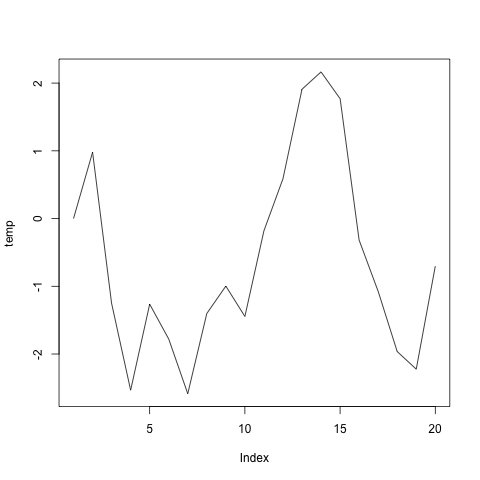
\includegraphics[width=\linewidth]{20-09-plot}
	\end{subfigure}
	\begin{subfigure}{0.23\textwidth}
		\centering
		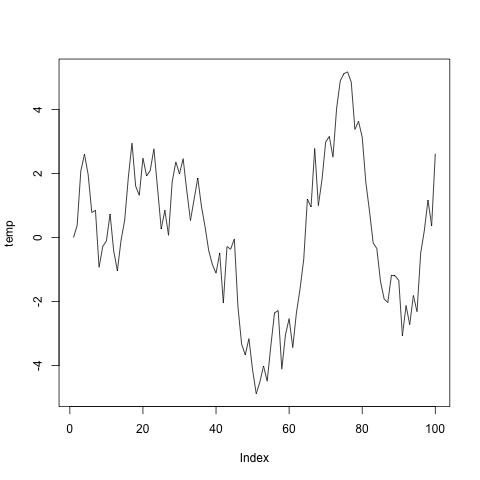
\includegraphics[width= \linewidth]{100-09-plot}
	\end{subfigure}
	\begin{subfigure}{0.23\textwidth}
		\centering
		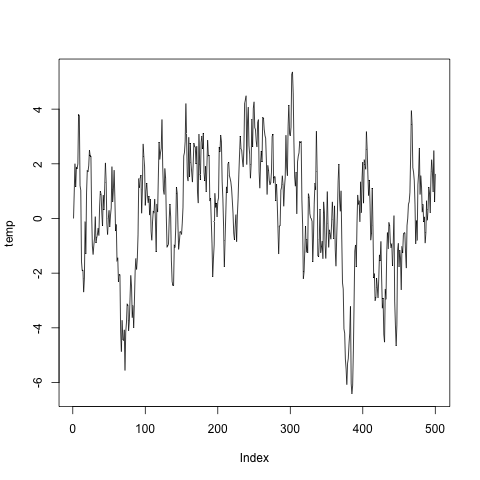
\includegraphics[width=\linewidth]{500-09-plot}
	\end{subfigure}
\caption{Time series plots for $\rho = 0.9$}
\end{figure}


For $T = 10$, $T = 20$ and $T = 100$, the process appears to have a trend while exhibiting a large amount of noise. $T = 500$ beings to resemble a random walk with a drift. None of these are correct diagnoses of the underlying process, however, with remains a zero-mean AR(1) process with an error term, $\epsilon_t$, of $N(0,1)$. The ACF for $T = 10$ is still showing no autocorrelation, while $T = 20$, $T = 100$ and $T = 500$ all show strong autocorrelation. The PACF for this process shows an AR(1) process for all but the shortest series.

\begin{figure}[htp]
	\centering
	\begin{subfigure}{0.23\textwidth}
		\centering
		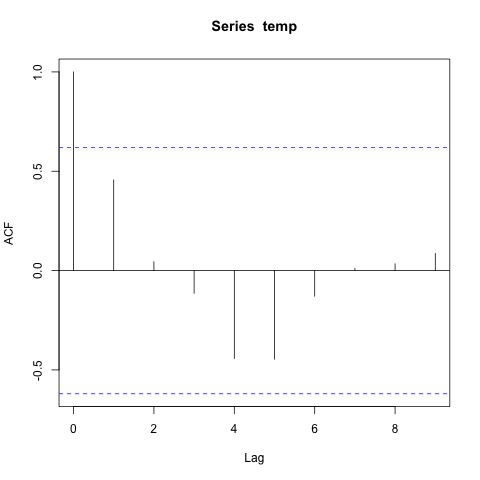
\includegraphics[width= \linewidth]{10-09-acf}
	\end{subfigure}
	\begin{subfigure}{0.23\textwidth}
		\centering
		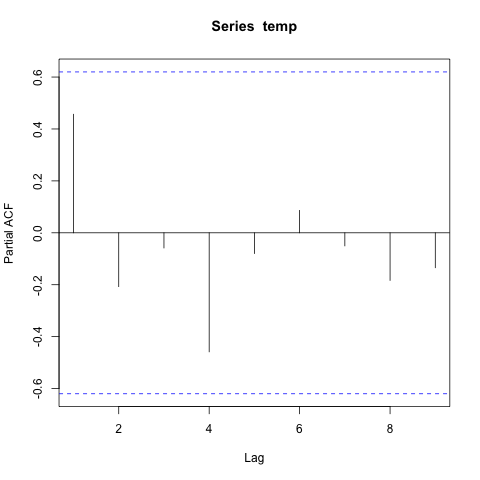
\includegraphics[width=\linewidth]{10-09-pacf}
	\end{subfigure}
	\begin{subfigure}{0.23\textwidth}
		\centering
		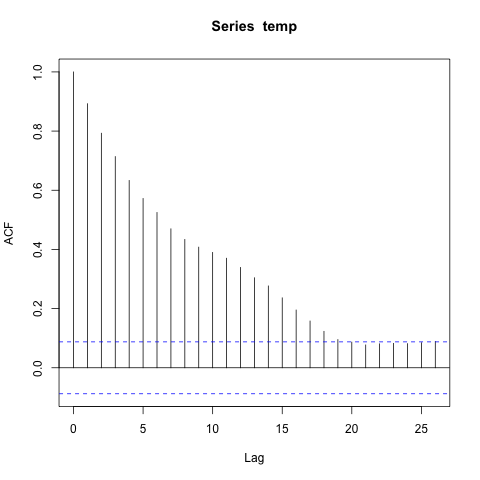
\includegraphics[width= \linewidth]{500-09-acf}
	\end{subfigure}
	\begin{subfigure}{0.23\textwidth}
		\centering
		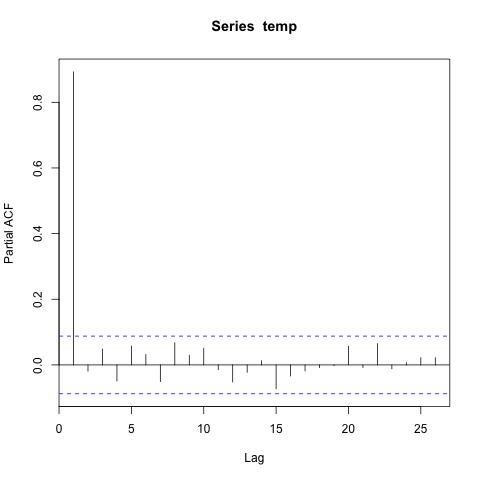
\includegraphics[width=\linewidth]{500-09-pacf}
	\end{subfigure}
	\caption{ACF and PACF plots for $\rho = 0.9$}
\end{figure}


Lastly, it would be prudent to demonstrate a unit root process over the same period of time. It is important to demonstrate the tangible difference between stationary data and non-stationary data in order to motivate the work that follows. The process is effectively a random walk, and this is proven when the process is differentiated, as the deterministic element is eliminated and the only remaining coefficient is the error term, which is a purely stochastic process, hence a random walk:


\begin{equation}
y_t = y_0 + \sum_{i=1}^{T}\epsilon_t
\end{equation}


As is known, a unit root process is an $AR$ process where the $\rho$ coefficient is equal to 1. As demonstrated above, such a process is purely stochastic and thus a random walk.


\begin{figure}[htp]
	\centering
	\begin{subfigure}{0.23\textwidth}
		\centering
		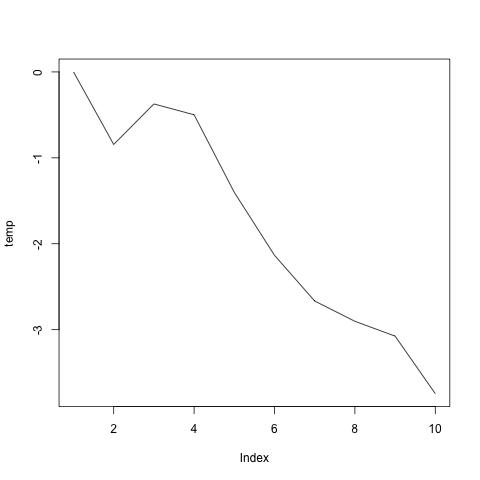
\includegraphics[width= \linewidth]{10-100-plot}
	\end{subfigure}
	\begin{subfigure}{0.23\textwidth}
		\centering
		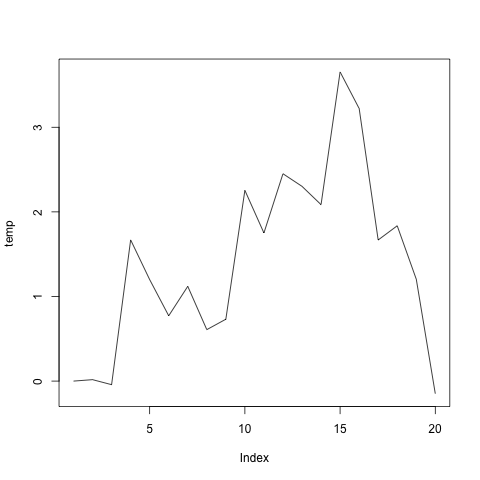
\includegraphics[width=\linewidth]{20-1-plot}
	\end{subfigure}
	\begin{subfigure}{0.23\textwidth}
		\centering
		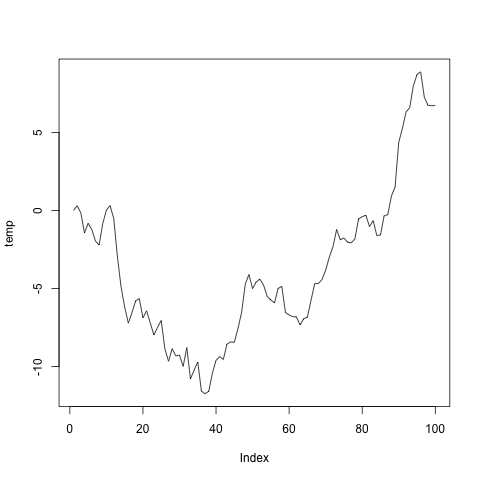
\includegraphics[width= \linewidth]{100-1-plot}
	\end{subfigure}
	\begin{subfigure}{0.23\textwidth}
		\centering
		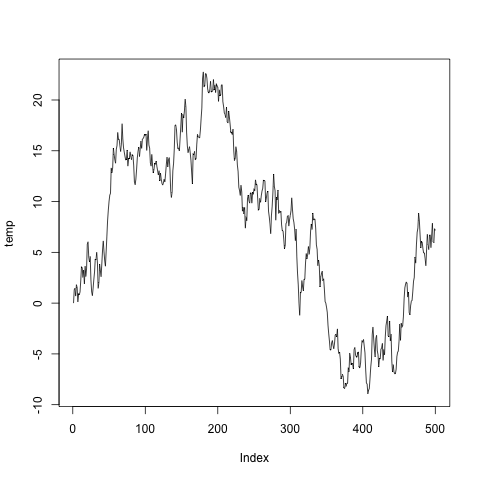
\includegraphics[width=\linewidth]{500-1-plot}
	\end{subfigure}
	\caption{Time Series plots for $\rho = 1$}
\end{figure}


The first interesting thing about the unit root process is that for a short time dimension (say $T = 10$ and $T = 20$), the process appears deterministic, much like the $T = 10$ and $T = 20$ processes of $\rho = 0.75$ and $\rho = 0.9$, which are actually stationary. This is important to note, as this highlights the difficulty faced by stationarity testing for short time series, which will be discussed in detail below. For longer series (say $T = 100$ and $T = 500$), the process is very clearly stochastic, with very abrupt deviations from a short term mean. While the ACF for $T = 10$ did not show autocorrelation (likely because of the small time dimension), $T = 20$, $T =100$ and $T = 500$ all showed a large amount of autocorrelation. When the PACF was used, all but the shortest series showed an $AR(1)$ process with correlations of above 0.8 for the first lag.

\begin{figure}[htp]
	\centering
	\begin{subfigure}{0.23\textwidth}
		\centering
		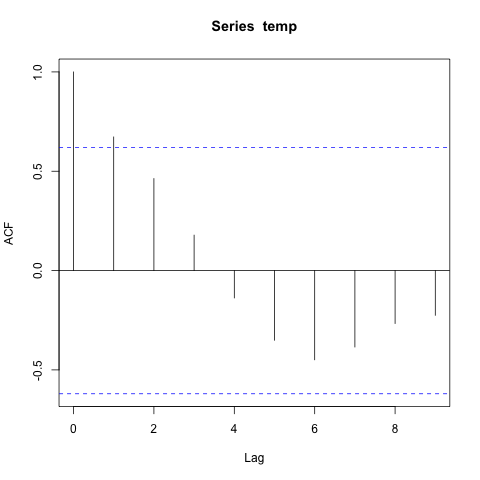
\includegraphics[width= \linewidth]{10-100-acf}
	\end{subfigure}
	\begin{subfigure}{0.23\textwidth}
		\centering
		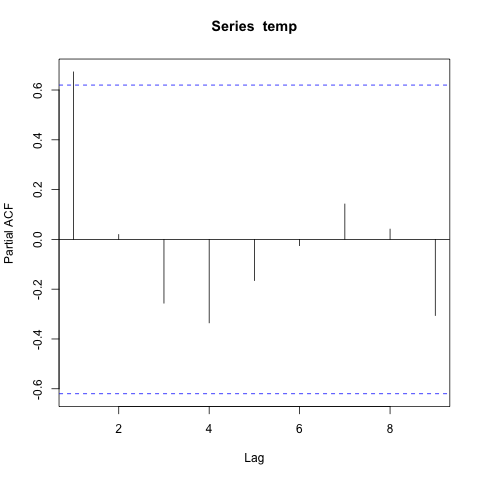
\includegraphics[width=\linewidth]{10-100-pacf}
	\end{subfigure}
	\begin{subfigure}{0.23\textwidth}
		\centering
		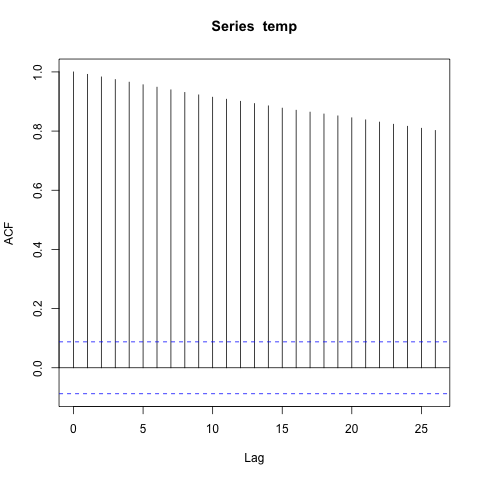
\includegraphics[width= \linewidth]{500-1-acf}
	\end{subfigure}
	\begin{subfigure}{0.23\textwidth}
		\centering
		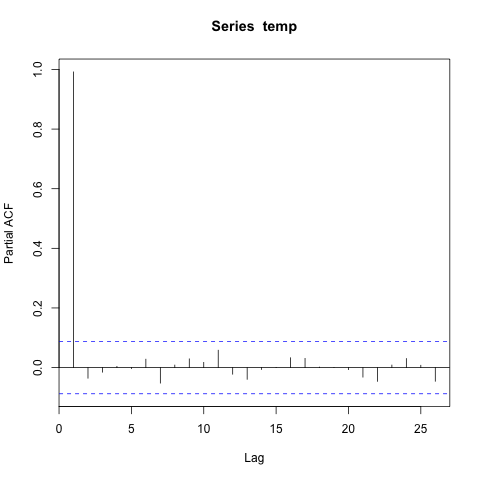
\includegraphics[width=\linewidth]{500-1-pacf}
	\end{subfigure}
	\caption{ACF and PACF for $\rho = 1$}
\end{figure}


Though the underlying process may be stochastic, a short sample of the process examined in isolation may appear and test as a deterministic process. This is visible with the ACF and PACF functions for the shortest series for all cases of $\rho$, where there is clearly not enough data to construct an accurate inference of the underlying data. Visually, the distinction between a stationary and non-stationary process is not large, especially for very short time series. The issue here is that the short dimension of the sample of the process means that the underlying process is not inherently determinable. A similar issue is understandably faced by stationarity testing, where a small sample does not expose enough of the process for correct inferences to be made.
